\documentclass[conference]{IEEEtran}
\IEEEoverridecommandlockouts
% The preceding line is only needed to identify funding in the first footnote. If that is unneeded, please comment it out.
\usepackage{cite}
\usepackage{amsmath,amssymb,amsfonts}
\usepackage{algorithmic}
\usepackage{graphicx}
\usepackage{textcomp}
\usepackage{xcolor}
\def\BibTeX{{\rm B\kern-.05em{\sc i\kern-.025em b}\kern-.08em
    T\kern-.1667em\lower.7ex\hbox{E}\kern-.125emX}}
\begin{document}

\title{CSCE 421 Final Project\\
}

\author{\IEEEauthorblockN{Jared Clifford}
\IEEEauthorblockA{\textit{827004032} \\
CSCE 421 \\
jcliff2000@tamu.edu}

}

\maketitle

\begin{abstract}
This paper describes the techniques used in order to create a Recursive Neural Network (RNN) to build a sequence to sequence model that takes 30 characters as input and estimates the next 10 characters as outputs. The model uses two Gated Recurrent Units (GRU) one as an encoder and one as a decoder. The model was trained on the enwik8 data set and was unable to accurately predict the next 10 letters averaging only 8\% accuracy.
\end{abstract}


\section{Introduction}
This document will discuss an overview of the which is a sequence to sequence neural network. A neural network (NN) is a deep learning model that consists of many connected activation functions with weights that starts with a given input that is then multiplied by weights to the next activation function where each connection between activation functions are given their own weight. The outputs for each activation function is then multiplied by the next connections weight and the pattern continues until the final activation function which acts as the output for the model[1]. An equation for the input to the activation function is shown below.
$$ f(x_1, x_2 ... x_3) = \Sigma_{i=1}^{n} w_i * x_i $$
\>In order to train neural nets a loss function is needed to calculate the correctness of the output compared to the expected output negative log likely-hood was used in this model to calculate the loss. In order to optimize the machine we must find what weights in each connection will lead to the smallest average loss. If we take the gradient for each node we can find the rate of change of the loss and since we want to decrease the loss we will subtract the gradient from the initial weight, but we don't want to update the weights too much so that they overshoot the minimum so we multiply the gradient by a learning rate that we decide[2]. So the rule for updating the weights is shown below
$$ w_i = w_i- lr\frac{L}{\partial w_i}$$
After each train the gradient is calculated and the weights are updated\\
For this model an RNN was used in order to predict due to the dependency's that languages have. RNNs are able to connect previous information to the present task due to the previous input being kept and passed through to the current input as shown in "fig 1".

\begin{figure}[htbp]
\centerline{\includegraphics{RNN.png}}
\caption{Example of how inputs are affected by the previous input[4]}
\label{fig1}
\end{figure}

With RNNs we will be able to build a model that can account for the dependencies in English language and predict the next letters through the use of GRUs. GRUs require two inputs, one is a variable passed into the model and the other is the hidden state that was produced by the GRU in the previous state. The GRU is comprised of a Reset Gate that handles the short term and an update gate that handles long term memory[5]. This allows the gate to be able to handle dependency's in language at both the word level and sentence level. However there is no internal memory in GRU making the long term memory not as favorable in some instances to other options such as long short term memory RNNs. To handle this we use an attention matrix. An attention matrix is useful in this case because it allows the model to have a connection to previous iterations that accumulate. Allowing the inputs to be affected by previous outcomes before it gets to the GRU[6].

\section{The Data}

\subsection{Data Set}
The data used in order to train, test, and validate the model is the Hutter Prize Wikipedia data set. The data is the first 100,000,000 bytes of a Wikipedia XML Dump that consists of 205 unique utf8 characters. However for the scope of this program only characters in the English language are used. This is decided based on limited computational resources, time, and readability. The XML had many lines that would not be useful to a model that needed to predict English text and often times could reduce the interpret-ability of the model due to the data set being written in a syntax that differs greatly from English. 

\subsection{Preprocessing the Data}
The first step to the preprocessing was to take in all the data from the data set, after that only the English characters (a-z) were selected, and all capitalized letters were changes to lower case. Accepting only the characters in the English alphabet helped to thin the large data set as even with only those characters being accepted the data was to large to run without parallelization. Another feature of excluding non alphabet characters was increased readability as non-alphanumeric characters were very common. After selecting specific characters the next step was to create a dictionary for all unique characters in order to somewhat normalize the data. Each character can now be indexed to a number between 0 and 26. This step was important as the encoder would only need 26 dimensions to properly encode the data where as if this step was not taken the largest value would have been 121 or the Unicode value for lowercase 'z' and the lowest value would have been 97 or lower case 'a'. That would have left the encoder having to encode the data into 26 data points into 121 length matrix with most of the indexes to be redundant. This saves the model both time and storage, which was greatly needed as even still running the model took hours to complete.

\subsection{Splitting Data}
After the data had been processed the next step was to split the data into test, training, and validation. due to the size of the data set not all of the data was used. At first when trying to use 80\% of the data resulted in extremely long run times and was not even able to handle 1\% of the data within an hour, because of this a large portion of the data was excluded in order to get some results, although the results would be less accurate. The train data set is comprised of 4000000 characters that create 100000 separate 40 length data points to be used and the test set is 1000000 characters that create 25000 data points to test with.

\section{The Model}
The model consists of an encoder and decoder both using GRUs. The decision to go with a GRU based model vs a long short term memory based model(LSTM) was due to the simplicity of GRUs and that they require less memory and are quicker to compute. Negative log likely hood loss function was used to calculate the loss and stochastic gradient decent was used as the optimizer for both the encoder and the decoder
\subsection{Encoder}
The encoder starts with embedding the inputs into an array of a hidden size, in this model a size of 50 was use as a compromise between wanting the encoder to properly have space to encapsulate important features, but not wanting it to be too large so that it doesn't slow down the model too much as there are a lot of data points to iterate through and the larger the matrix the more gradients have to be calculated. The embedded array then is fed into the GRU with the previous embedded array, and the first element is fed into the GRU with an empty array. Once the final character of the data point is fed through the final array is passed into the decoder.
\subsection{Decoder}
The decoder contains an attention matrix, since the input token range is 26 which is the same as the range of the output the size of this matrix is 26 by 26. When training the decoder uses the previous expected values when testing it will use the previous predicted value. It embeds the value and then applies a linear transformation across the embedded matrix and hidden matrix from the previous iteration if there was not previous iteration the hidden matrix is all zeros. The result of that transformation gets put into a soft max that each value can be interpreted as a probability. Those values then get linearly combined with the attention matrix. The next layer has an activation function of relu and after that they go through the GRU. Finally the output is calculated in the last layer using the log of the softmax to generate a 26 matrix to be out put along with the hidden layer that will be used by the next value to be estimated.

\section{Results}

The model was ran with 100000 data points for training and 25000 data points to be tested after each epoch. The program was set to run 15 epochs. The model was finished training after 11 hours and 28 mins. The model was unsuccessful at predicting the next characters as the train loss barely decreased and accuracy became stagnant around 8\% accuracy, which is better than a random guess however that means less than one letter was correct per data point. While the test data loss and accuracy fluctuated much more than the test it was also around the same range as the train loss and accuracy. Below are the graphs for the average loss "Fig. 2" and accuracy "Fig. 3" for the epochs.

\begin{figure}[htbp]
\centerline{\includegraphics{loss.png}}
\caption{Average loss per epoch}
\label{fig1}
\end{figure}

\begin{figure}[htbp]
\centerline{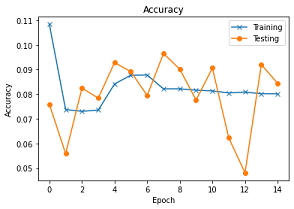
\includegraphics{accuracy.png}}
\caption{Average accuracy per epoch}
\label{fig2}
\end{figure}

After the test has finished a function call to evaluate selects a random data point to take 40 characters from and returns the predicted 10 which can be compared to the expected 10 characters. The results of a few calls are shown in the table below in "Table 1"

\begin{table}[htbp]
\caption{Evaluating Model Predictions}
\begin{center}
\begin{tabular}{|c|c|c|}
\hline
\textbf{Input}&\textbf{Expected} & \textbf{Predicted} \\
\hline
rmainly aimed at os and windows thou&gh it develo&nededddded \\
\hline
s concerns but stating his intentio&n to continu&ndndindndn \\
\hline
ive copy no registratio nrequired l & trefgtinth&iiiiiiiiii \\
\hline
lly went into enforced liquidation&and were ign&djdddddddd\\
\hline
\end{tabular}
\label{tab1}
\end{center}
\>*spaces were added to Input and Expected to improve readability
\end{table}

The predicted outputs seem to have little correlation to the input and are far off from the output. The model mostly returns commonly seen characters and is most likely just guessing characters that are seen frequently such as "i"s and "d"s which appear very often in id tags in the XML

\section{Conclusion}

In this work I created a sequence to sequence model that was suposed to be able to accurately predect the next ten characters given 30. The accuracy shows that the model was not successful and predicting, and rather seems to guess one to two common letters. Although this model did not perform well there many be many reasons for that. Many limitations set back the ability to create a model that will accurately predict characters. Time was ultimately a limiting factor when developing the model as well as not being able to parallelize the model thus only decreasing the ability to run more data. 
\subsection{Possible Reasons of Failure}
The model was only with 100,000 datapoints with 15 epochs however this was only 4\% of the dataset. Another problem with the dataset that was not properly handled was leaving in XML tags despite taking out other symbols. Not removing the XML tags could have created more confusion for the machine as it is getting some inputs that make no sense therefore it can have a harder time detecting what patterns occur in language. A GRU was used instead of an LSTM due to GRUs being less resource intensive and quicker[3], however that trade-off was definitely a limiting factor when trying to increase the accuracy. Another issue with the model was wanting to use less dimensions in order to limit the amount of calculations when calculating gradients. This decision also came at a cost to accuracy. Lastly the learning rate could have been too small and had no momentum. The gradient could have stalled in a local minimum and therefore was not able to converge properly
\subsection{Moving Forward}
Although the model did not perform well, there could be some alterations that might help. If time was not an issue perhaps implementing the fixes described above would be able to fix the issues with the machine not being able to learn properly



\begin{thebibliography}{00}
\bibitem{b1} “Deep learning in neural networks: An overview,” science direct. pp. 85–117, Jan-2015. 
\bibitem{b1} V. Bushaev, “How do we 'train' neural networks ?,” Medium, 22-Oct-2018. [Online]. Available: https://towardsdatascience.com/how-do-we-train-neural-networks-edd985562b73. [Accessed: 13-Dec-2021].
\bibitem{b1}V. Lendave, “LSTM vs gru in recurrent neural network: A comparative study,” Analytics India Magazine, 27-Aug-2021. [Online]. Available: https://analyticsindiamag.com/lstm-vs-gru-in-recurrent-neural-network-a-comparative-study/. [Accessed: 13-Dec-2021]. 
\bibitem{b1}C. Olah, “Understanding LSTM networks,” Understanding LSTM Networks -- colah's blog. [Online]. Available: https://colah.github.io/posts/2015-08-Understanding-LSTMs/. [Accessed: 14-Dec-2021]. 
\bibitem{b1}S. Saxena, “Gated recurrent unit: Introduction to Gated Recurrent Unit(GRU),” Analytics Vidhya, 18-Mar-2021. [Online]. Available: https://www.analyticsvidhya.com/blog/2021/03/introduction-to-gated-recurrent-unit-gru/. [Accessed: 14-Dec-2021]. 
\bibitem{b1}N. Adaloglou, “How attention works in Deep learning: Understanding the attention mechanism in sequence models,” AI Summer, 19-Nov-2020. [Online]. Available: https://theaisummer.com/attention/. [Accessed: 14-Dec-2021]. 
\end{thebibliography}


\end{document}
